\section{Operation Description}

Figure \ref{fig:functional_flow_block_diagram} shows the functional flow block diagram of SitaWare Civilian. The figure depicts the top-level functionality of the system where a user initially deploys the mobile SitaWare Civilian HQ. After system initialization the user is presented to the COP and simultaneously the system starts a "thread" for collecting various static and dynamic data. The "thread" keeps the COP updated with the collected data along with registered events from other users of the system. It is at all times possible for the user to dispatch orders to the other users. 

\begin{figure}[H]
\centering
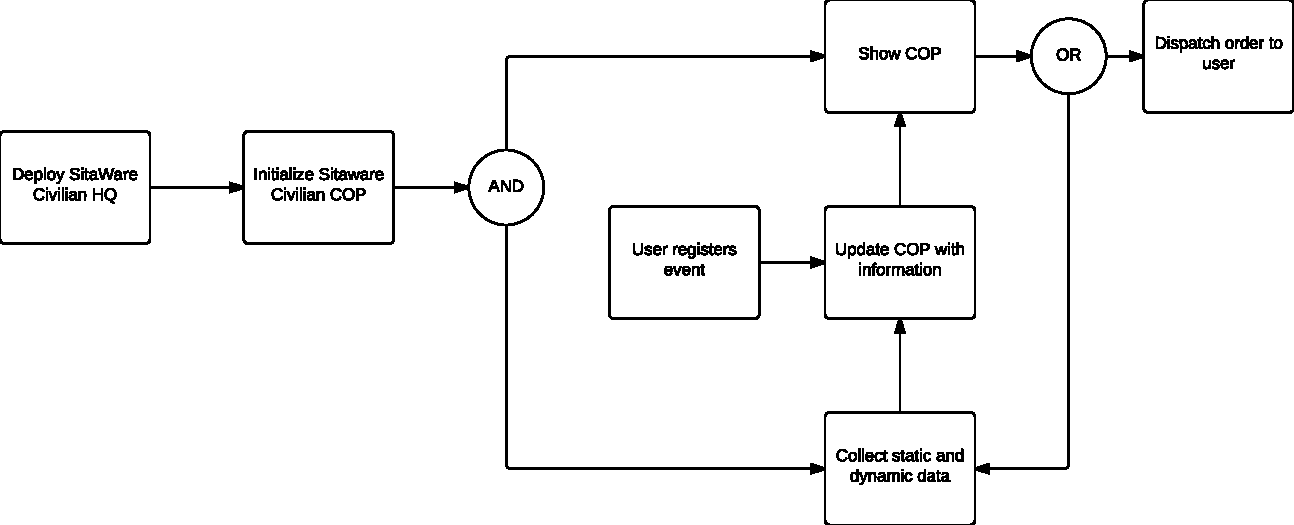
\includegraphics[width=0.95\textwidth]
{billeder/functional_flow_block_diagram.pdf}
\caption{Functional flow block diagram.}
\label{fig:functional_flow_block_diagram}
\end{figure}